\section{Deriving error bounds}
\label{sec:error-bounds}
%We bound the error induced by relaxation on two representative sketches.
Section~\ref{ssec:theta-analysis} discusses the error introduced to the
expected estimation and RSE of the KMV $\Theta$ sketch.
Section~\ref{ssec:quantiles-error-analysis} analyses the PAC Quantiles sketch.
The full paper~\cite{rinberg2019fast} contains mathematical derivations used throughout this section. 

\subsection{$\Theta$ error bounds}
\label{ssec:theta-analysis}

We bound the error introduced by an $r$-relaxation of the $\Theta$ sketch. Given
Theorem~\ref{lemma:opt-genereic-strong}, the optimised concurrent sketch's error is bounded
by the relaxation's error bound for $r=2N$$b$. We consider strong and weak adversaries,
${\mathcal{A}}_s$ and ${\mathcal{A}}_w$, resp. For the strong adversary we are able to show only numerical
results, whereas for the weak one we show closed-form bounds. The results are summarised in Table~\ref{table:Theta-Error-Summary}.
Our analysis relies on known results from order statistics~\cite{david2004order}.
It focuses on long streams, and assumes $n>k+r$.

%\begin{table}[H]
%    \begin{tabular}{c|cc|cc|cc}
%                      & \multicolumn{2}{c|}{Sequential sketch} & \multicolumn{2}{c|}{Strong adversary ${\mathcal{A}}_s$} & \multicolumn{2}{c}{Weak adversary ${\mathcal{A}}_w$}   \\[5pt]
%                      & Closed-form& Numerical& \multicolumn{2}{c|}{Numerical} & \multicolumn{2}{c}{Closed-form}   \\[5pt]
%                      \hline
%    Expectation & $n$        & $2^{15}$        & \multicolumn{2}{c|}{$2^{15} \cdot 0.995$}          & \multicolumn{2}{c}{$n\frac{k-1}{k+r-1}$} \\[5pt]
%    RSE & $\leq \frac{1}{\sqrt{k-2}}$        & $\leq 3.1\%$        & \multicolumn{2}{c|}{$\leq 3.8\%$}           & \multicolumn{2}{c}{$\leq 2\frac{1}{\sqrt{k-2}}$}         
%    \end{tabular}
%    \caption{Analysis of $\Theta$ sketch with numerical values for $r=8, k=2^{10}, n=2^{15}$.}
%    \label{table:Theta-Error-Summary}
%\end{table}

\begin{table*}[!ht]
    % Table content (and caption)
    \begin{tabular}{c|cc|cc|cc}
        & \multicolumn{2}{c|}{Sequential sketch} & \multicolumn{2}{c|}{Strong adversary ${\mathcal{A}}_s$} & \multicolumn{2}{c}{Weak adversary ${\mathcal{A}}_w$}   \\%[5pt]
        & Closed-form& Numerical& \multicolumn{2}{c|}{Numerical} & \multicolumn{2}{c}{Closed-form}   \\%[5pt]
        \hline
        Expectation & $n$        & $2^{15}$        & \multicolumn{2}{c|}{$2^{15} \cdot 0.995$}          & \multicolumn{2}{c}{$n\frac{k-1}{k+r-1}$} \\%[5pt]
        RSE & $\leq \frac{1}{\sqrt{k-2}}$        & $\leq 3.1\%$        & \multicolumn{2}{c|}{$\leq 3.8\%$}           & \multicolumn{2}{c}{$\leq 2\frac{1}{\sqrt{k-2}}$}         
    \end{tabular}
    \caption{Analysis of $\Theta$ sketch with numerical values for $r=8, k=2^{10}, n=2^{15}$.}
    \label{table:Theta-Error-Summary}
\end{table*}

We would like to analyse the distribution of the $k^{th}$ largest element in the 
stream that the relaxed sketch processes, as this determines the result returned by the algorithm. 
We cannot use order statistics to analyse this 
because the adversary alters the stream and so the stream seen by the algorithm is not random.
%the $k^{th}$ largest element in the stream is not a random variable. 
However, the stream of hashed unique elements seen by the adversary \emph{is} random. 
Furthermore, if the adversary hides from the algorithm $j$ elements 
smaller than $\Theta$, then the $k^{th}$ largest element in the stream seen
by the  sketch is the $(k+j)^{th}$ largest element in the original stream seen by the adversary. 
This element is a random variable and therefore we can apply order statistics to it.  

We thus model the hashed unique elements in the stream $A$ processed before a given
query as a set of $n$ labelled iid random variables $A_1,\dots,A_n$, taken uniformly 
from the interval $[0,1]$. Note that
$A$ is the stream observed by the reference sequential sketch, and 
also by adversary that hides up to $r$ elements from the relaxed sketch. 
Let $M_{(i)}$ be the $i^{th}$ minimum value among the $n$ random variables $A_1,\dots,A_n$.

Let $est(x) \triangleq \frac{k-1}{x}$ be the estimate computation
with a given $x=\Theta$ (line~\ref{l:update-est} of Algorithm~\ref{alg:composable-theta}).
The sequential (non-relaxed) sketch returns $e=est(M_{(k)})$.
It has been shown that the sketch is unbiased~\cite{KMV}, i.e., $E[e]=n$ the number of unique elements,
and $RSE[e]\leq \frac{1}{\sqrt{k-2}}$.
The \emph{Relative Standard Mean Error (RSME)} is the error relative to the mean, formally defined in
the full paper~\cite{rinberg2019fast}.
%the supplementary material Section~\ref{ssec:RSE-RMSE}.
Because this sketch is unbiased, \emph{RSE}$[e]=$\emph{RSME}$[e]$.


In a relaxed history, the adversary chooses up to $r$ variables to hide from the given query so as to maximise its
error. It can also re-order elements, but the state of a $\Theta$ sketch after a set of updates
is independent of their processing order. Let $M^r_{(i)}$ be the $i^{th}$ minimum value among
the hashes seen by the query, i.e., arising in updates that precede the query in the relaxed history.
The value of $\Theta$ is $M^r_{(k)}$, which is equal to $M_{(k+j)}$ for some $0 \leq j \leq r$.
We do not know if the adversary can actually control $j$,
but we know that it can impact it, %and so to bound the error, we can take the worst possible $j$.
%While an arbitrary set of $r$ updates is hidden, in the $\Theta$ sketch,
%only hidden elements that impact $j$ (have hashes smaller than $M^r_{(k)}$)
%affect the query.
and so for our error analysis, we consider strictly stronger adversaries --
we allow both the weak and the strong adversaries to choose the number of hidden
elements $j$. Our error analysis gives an upper bound on the error induced by our adversaries.
Note that the strong adversary can choose $j$ based on the coin flips,
while the weak adversary cannot, and therefore chooses the same $j$ in all runs.
%The strong adversary knows the hash function and can select $j$ adaptively; the
%weak adversary does not and therefore chooses the same $j$ in all runs.  
%Note that $j$ counts only hidden elements smaller
%than $\Theta$; others are inconsequential.
In the full paper~\cite{rinberg2019fast} we show that
the largest error is always obtained either for $j=0$ or for $j=r$. 
\begin{figure}[b]
%\begin{wrapfigure}{r}{0.4\textwidth}
    \begin{center}
        %\vspace{-0.4in}
        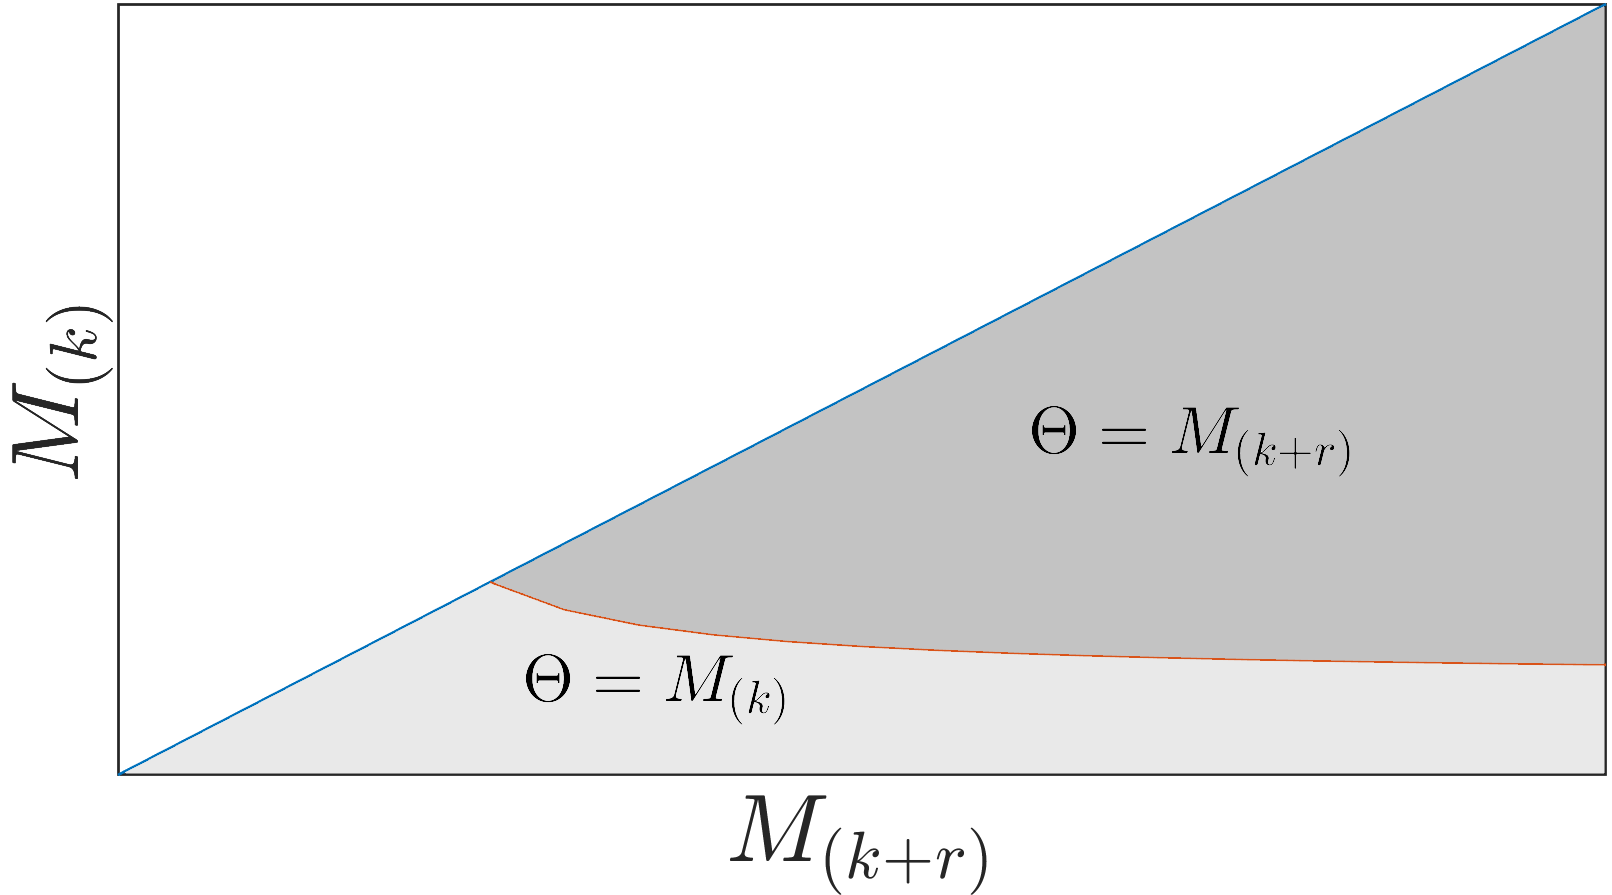
\includegraphics[width=0.38\textwidth]{images/areaGraph.png}
        %\vspace{-0.2in}
    \end{center}
    \caption{Areas of $M_{(k)}$ and $M_{(k+r)}$. In the dark gray 
    ${\mathcal{A}}_s$ induces $\Theta=M_{(k+r)}$, and in the light gray, $\Theta=M_{(k)}$. The white
    area is not feasible.} %\vspace{-0.1in}
    \label{fig:areaGraph}
%\end{wrapfigure}
\end{figure}

Given an adversary $\mathcal{A}$ that induces an approximation $e_{\mathcal{A}}$, in the full paper~\cite{rinberg2019fast} we prove
the following bound:
%Lemma~\ref{lemma:theta-adversary-bound} in the supplementary material Section~\ref{ssec:theta-error-bounds} proves the following bound:
\begin{align*}
    \text{RSE}[e_{\mathcal{A}}] \leq \sqrt{\frac{\sigma^2(e_{\mathcal{A}})}{n^2}} + \sqrt{\frac{(E[e_{\mathcal{A}}] - n)^2}{n^2}}.
\end{align*}

\paragraph{Strong adversary ${\mathcal{A}}_s$} The strong adversary knows the coin flips in advance, and thus chooses
$j$ to be $g(0, r)$, where $g$ is the
choice that maximises the error:
\begin{align*}
    g(j_1, j_2) \triangleq \argmax_{j \in \left\{j_1, j_2\right\}} \abs{\frac{k-1}{M_{(k+j)}} - n}.
\end{align*} 

\begin{figure}[b]
%\begin{wrapfigure}{l}{0.4\textwidth}
    \begin{center}
        %\vspace{-0.2in}
        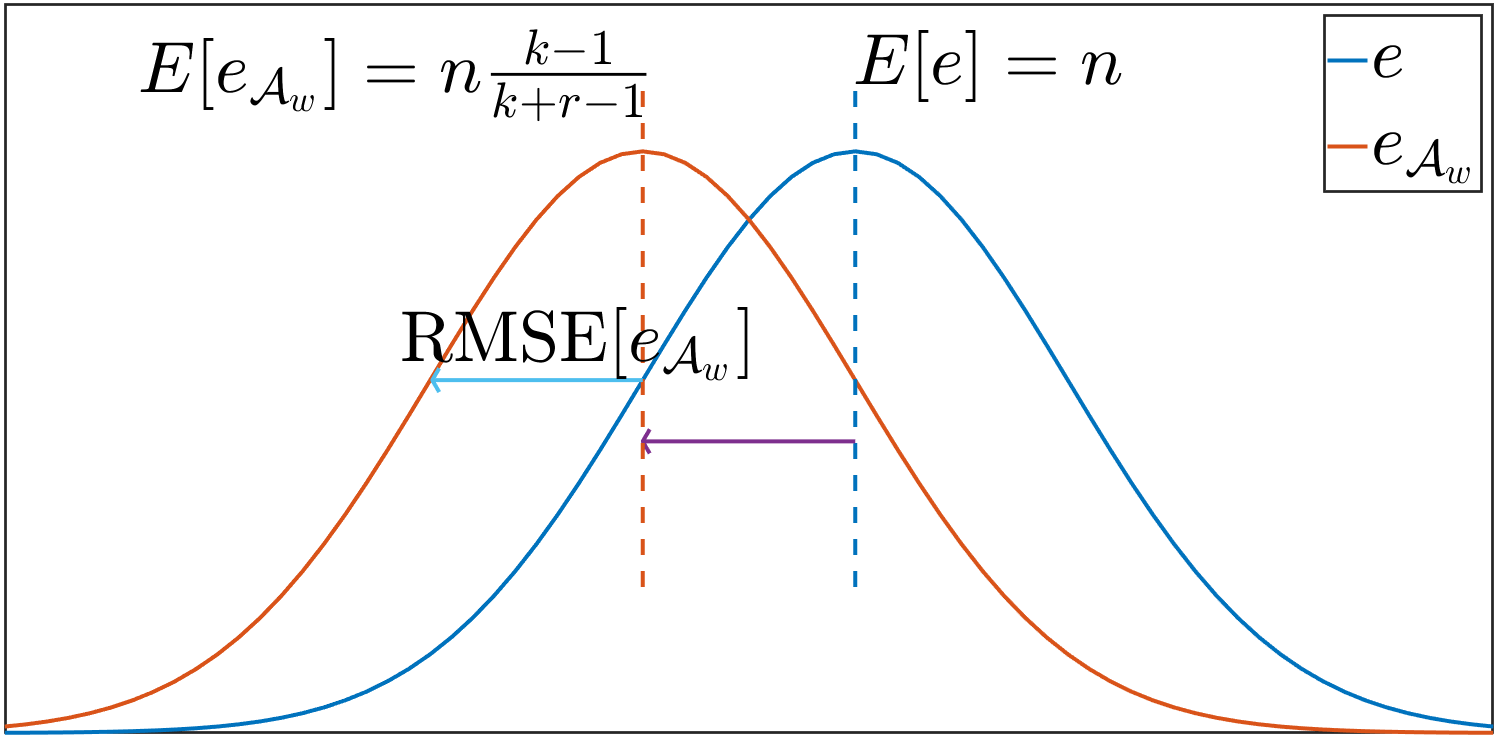
\includegraphics[width=0.39\textwidth]{images/thetaGraph.png}
        %\vspace{-0.2in}
    \end{center}
    \caption{Distribution of estimators $e$ and $e_{{\mathcal{A}}_w}$. The RSE of $e_{{\mathcal{A}}_w}$ with regards to $n$ is bounded
    by the relative bias plus the RMSE of $e_{{\mathcal{A}}_w}$.}%\vspace{-0.2in}}
    \label{fig:thetaGraph}
%\end{wrapfigure}
\end{figure}

In Figure~\ref{fig:areaGraph} we plot the regions where $g$ equals $0$
and $g$ equals $r$, based on their possible combinations of values. The estimate
induced by ${\mathcal{A}}_s$ is $e_{{\mathcal{A}}_s} \triangleq \frac{k-1}{M_{(k+g(0,r))}}$. The expectation
and standard error of $e_{{\mathcal{A}}_s}$ are calculated by integrating over the gray areas
in Figure~\ref{fig:areaGraph}
using their joint probability function from order statistics. In the full paper~\cite{rinberg2019fast} we give
%Equations \ref{eq:strong-expectation}
%and \ref{eq:strong-se-bound} in the supplementary material Section~\ref{ssec:theta-error-bounds} give
the formulas for the expected estimate and its RSE bound, resp. We do not have
closed-form bounds for these equations. Example numerical results are
shown in Table~\ref{table:Theta-Error-Summary}.

\paragraph{Weak adversary ${\mathcal{A}}_w$} Not knowing the coin flips, ${\mathcal{A}}_w$ chooses $j$
that maximises the expected error for a random hash function:
$E[n-est(M^r_{(k)})]=E[n-est(M_{(k+j)})]=n-n\frac{k-1}{k+j-1}$. Obviously this
is maximised for $j=r$. The orange curve in Figure~\ref{fig:thetaGraph} depicts
the distribution of $e_{{\mathcal{A}}_w}$, and the distribution of $e$ is shown in blue.

%Not knowing the coin flips, what ${\mathcal{A}}_w$ will
%attempt to maximise the expected error of the query \inred{by doing what?}:
%\begin{align*}
%    E[n-est(M^r_{(k)})]=E[n-est(M_{(k+j)})]=n-n\frac{k-1}{k+j-1}
%\end{align*}

%For some $0 \leq j \leq r$. Note that the error is maximised for $j=r$.
%As the adversary does not know the coin flips, it will attempt
%to maximise the number of updates stuck in the local buffers, as an
%update in the local buffers has a hash value is lower than $\Theta$ (or rather lower than $\Theta$
%after the last propagation). We can therefore bound the error induced by this adversary by an
%adversary $\hat{{\mathcal{A}}}_w$ that always hides $r$ elements smaller than $\Theta$, thus forcing
%$M^r_{(k)}=M_{(k+r)}$. The orange curve in Figure~\ref{fig:thetaGraph} depicts
%the distribution of $e_{\hat{{\mathcal{A}}}_w}$, and the distribution of $e$ is shown in blue.

In the full paper~\cite{rinberg2019fast},
%In Equation~\ref{eq:theta-rse-weak-bound} in the supplementary material Section~\ref{ssec:theta-error-bounds} 
we show that the RSE
is bounded by $\sqrt{\frac{1}{k-2}} + \frac{r}{k-2}$ for $\hat{{\mathcal{A}}}_w$, and therefore so
is that of ${\mathcal{A}}_w$.
Thus, whenever $r$ is at most $\sqrt{k-2}$, the RSE of the relaxed
$\Theta$ sketch is coarsely bounded by
twice that of the sequential one. And in case $k \gg r$, the addition to the $RSE$ is negligible.

\subsection{Quantiles error bounds}
\label{ssec:quantiles-error-analysis}

%\begin{wraptable}{c}{0pt}
%    \begin{tabular}{c|ccc}
%    Quantile        & Sequential                                   & Weak adversary ${\mathcal{A}}_w$ \\[5pt]
%    \hline
%    $\phi \leq 0.5$ & $\phi n \pm \epsilon n$ & $\phi n + (1-\phi)r \pm \epsilon(n - r)$ \\[5pt]
%    $\phi > 0.5$    & $\phi n \pm \epsilon n$ & $\phi n -\phi r \pm \epsilon(n - r)$
%    \end{tabular}
%    \caption{Quantiles sketch: Result range with probability $1-\delta$, for sequential sketch and $r$-relaxation with weak adversary,
%    and $\epsilon_r=\epsilon - \frac{r \epsilon}{n} + \frac{r}{n}$.}
%    \label{table:Quantiles-Error-Summary}
%\end{wraptable}

\iffalse
\begin{wraptable}{c}{0pt}
    \begin{tabular}{c|ccc}
    Quantile        & Sequential                                   & Weak adversary ${\mathcal{A}}_w$ \\[5pt]
    \hline
    $\phi $ & $\phi n \pm \epsilon n$ & $\phi n \pm \left(\epsilon - \frac{r \epsilon}{n} + \frac{r}{n}\right) n$ 
    \end{tabular}
    \caption{Quantiles sketch: Result range with probability $1-\delta$, for sequential sketch and $r$-relaxation with weak adversary,
    and $\epsilon_r=\epsilon - \frac{r \epsilon}{n} + \frac{r}{n}$.}
    \label{table:Quantiles-Error-Summary}
\end{wraptable}
\fi

We now analyse the error for any implementation of the sequential Quantiles sketch, provided that the sketch is
\emph{PAC}, meaning that a query for quantile $\phi$
returns an element whose rank is between $(\phi-\epsilon)n$ and $(\phi+\epsilon)n$ with 
probability at least $1-\delta$ for some parameters $\epsilon$ and $\delta$. We show that the $r$-relaxation of
such a sketch returns an element whose rank is in the range $(\phi \pm\epsilon_r)n$ with probability at
least $1-\delta$ for $\epsilon_r=\epsilon - \frac{r \epsilon}{n} + \frac{r}{n}$.

%The results are summarised in Table~\ref{table:Quantiles-Error-Summary}.

Although the desired summary is order agnostic here too, Quantiles sketch implementations (e.g., \cite{Agarwal:2012})
are sensitive to the processing order. In this case, advanced knowledge of the coin flips can increase the error
already in the sequential sketch. Therefore, we do not consider a strong adversary, but rather discuss only the weak one.
Note that the weak adversary attempts to maximise $\epsilon_r$.

Consider an adversary that knows $\phi$ and chooses to hide
$i$ elements below the $\phi$ quantile and $j$ elements above it, such that $0\leq i+j\leq r$. The rank of the element
returned by the query among the $n-(i+j)$ remaining elements is in the range 
$\phi(n-(i+j)) \pm \epsilon(n-(i+j))$.
There are $i$ elements below this quantile that are missed, and therefore its rank in the original stream is in the range:
\begin{equation}
    \left[ (\phi-\epsilon)(n-(i+j)) + i , (\phi+\epsilon)(n-(i+j)) + i \right].
    \label{eq:rank-range}
\end{equation}

This can be rewritten as:
\begin{equation}
\begin{split}
    [\phi n - (\phi j - (1-\phi)i+\epsilon(n-(i+j))), \\
    \phi n + ((1-\phi)i - \phi j +\epsilon(n-(i+j))) ] 
\end{split}
    \label{eq:rank-range-2}
\end{equation}

\iffalse

\begin{wrapfigure}{r}{0.3\textwidth}
    \begin{center}
        %\vspace{-0.2in}
      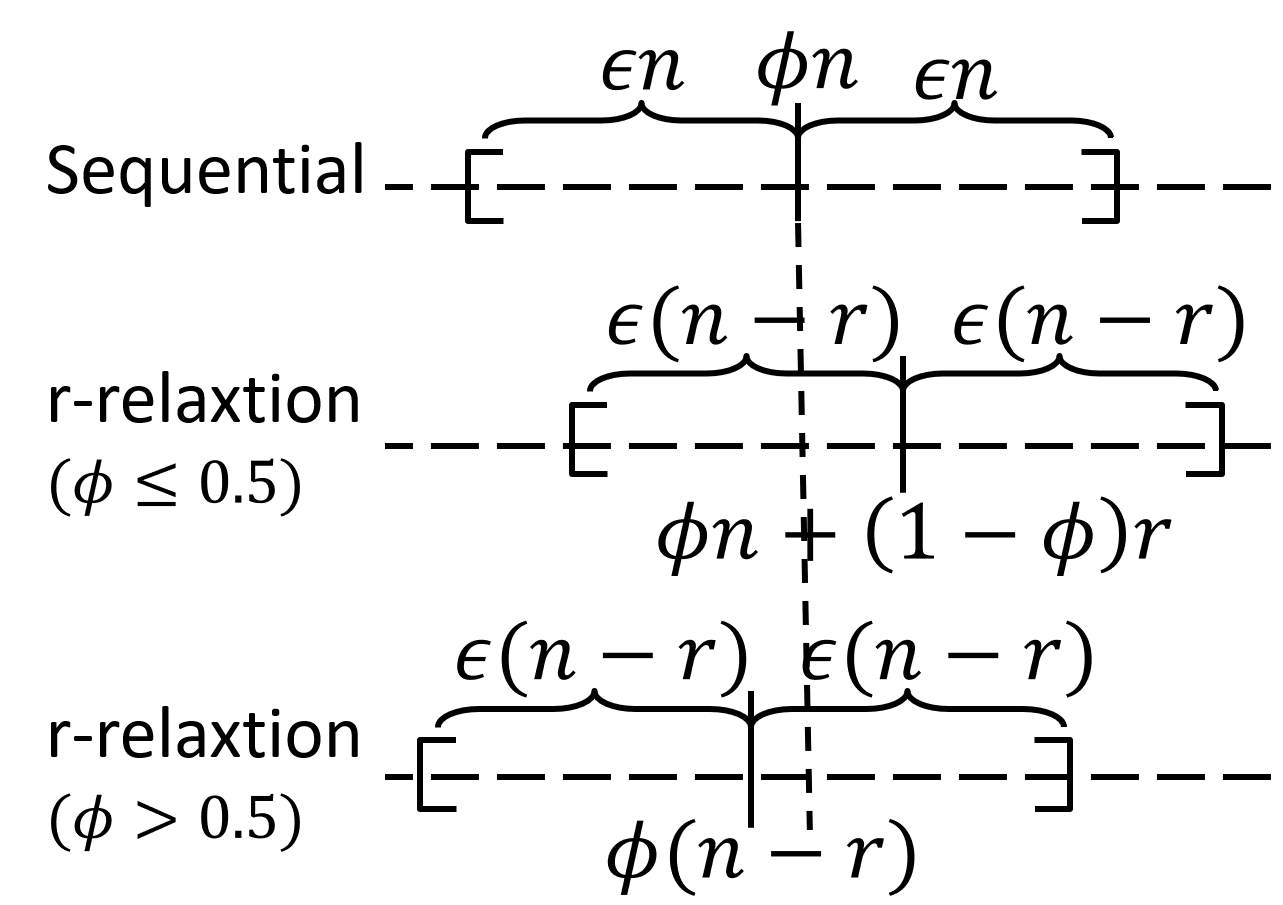
\includegraphics[width=0.29\textwidth]{images/quantilesRelaxtionRanges.png}
      %\vspace{-0.2in}
    \end{center}
    \caption{Ranges where the result of a query($\phi$) to
        a Quantiles sketch resides with probability $1-\delta$;
        for a sequential sketch and an $r$-relaxation. \vspace{0.2in}}
    \label{fig:quantiles-range}
\end{wrapfigure}

Note that this interval is symmetric around $\phi(n-(i+j)) + i$.
The adversary attempts to maximise the distance of the edges of this interval from the true rank,
(i.e., maximise $\epsilon_r$). The distance between the central points is:
\begin{align*}
    \abs{\phi n + (1-\phi)i - \phi j - \phi n}=\abs{(1-\phi)i - (\phi)j}.
\end{align*}
Given that $0\leq i+j\leq r$, we show that this expression is maximised
for $i+j=r$.
This is proven in the full paper~\cite{rinberg2019fast}.
%This is proven in Claim~\ref{claim:sum-r} in the supplementary material Section~\ref{ssec:quantiles-sketch-error-bounds}.
By substituting $j=r-i$ into the error formula, we get:
\begin{align*}
    \abs{(1-\phi)i - (\phi)(r-i)}=\abs{i - \phi r}.
\end{align*}
As $0\leq \phi \leq 1$, the following claim follows immediately:
\begin{claim}
    For $\phi \leq 0.5$ the adversary maximises the distance by choosing $i=r$ (and therefore $j=0$)
    and for $\phi > 0.5$ the adversary maximises the error by choosing $i=0$ (and therefore $j=r$).
    \label{clm:quantiles-relaxation-choice}
\end{claim}

\fi
In the full paper~\cite{rinberg2019fast}, we
%In Lemma~\ref{lemma:quantiles-weak-adversary} in the supplementary material Section~\ref{sec:appendix-error-bounds} we
show that the $r$-relaxed sketch returns an element whose rank is
between $(\phi-\epsilon_r)n$ and $(\phi+\epsilon_r)n$ with probability at
least $1-\delta$, where $\epsilon_r=\epsilon - \frac{r \epsilon}{n} + \frac{r}{n}$. Thus
the impact of the relaxation diminishes as $n$ grows.
%The ranges are illustrated in Figure~\ref{fig:quantiles-range}.